\subsection{Eigenschaften der Kinect} 
\begin{figure}[htbp] 
  \centering
     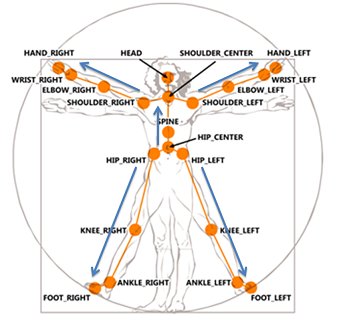
\includegraphics[width=0.7\textwidth]{skeletal.png}
  \caption{Gelenkpunkte die mit der Kinect getrackt werden können}
  \label{fig:Bild1}
\end{figure}
\cite{skeletal}
	Wir stellen in diesem Abschnitt nur die für uns interessanten Eigenschaften und Möglichkeiten der Kinect vor (hinsichtlich unserer Aufgabe und der Rahmenbedingungen). Die Kinect erkennt visuell den 3D-Raum vor sich. Dabei werden Personen als solche detektiert und konfidenzbasiert mit einem primitiven und grobgranularen Skelett ausgestattet. Dieses Tracking ist für bis zu sechs Personen zeitgleich möglich. Weiterhin wird für beide Hände einer getrackten Person ein \glqq Handzustand\grqq~erkannt, nämlich ob die Hand offen oder geschlossen ist, oder die sogenannte Lassogeste gebildet wird (etwa nur zwei Finger ausgestreckt). Kann einer Hand keiner dieser Zustände zugeordnet werden, ist ihr Status unbekannt. Diese Daten (Skelett und Status pro getrackter Person) können unter Verwendung der USB-Schnittstelle und des Kinect-SDKs abgegriffen werden. Sie werden dafür 30 mal in der Sekunde zur Verfügung gestellt.